\chapter[SCP-023 黑煞星]{
    SCP-023 Black Shuck\\
    SCP-023 黑煞星
}

\label{chap:SCP-023}

\begin{figure}[H]
    \centering
    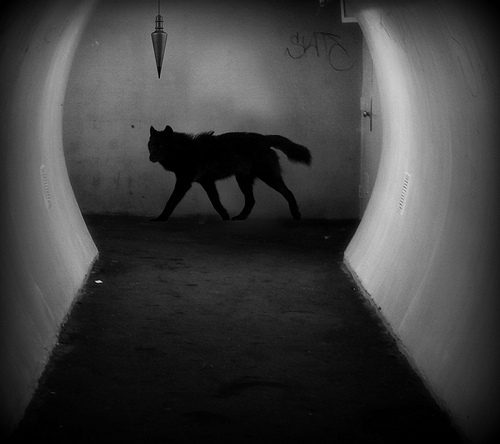
\includegraphics[width=0.5\linewidth]{images/SCP-023.jpg}
    \caption*{SCP-023于SCP-███逃脱事件中收容于暂时收容区}
\end{figure}

\bb{项目编号:}SCP-023

\bb{项目等级:}Euclid

\bb{特殊收容措施:}\dd{SCP-023应收容于一间5X5米的标准收容单位内。} SCP-023收容于Site-██的一处收容区,该区结构为两道回廊交错构成的叉状建物,并延边缘围起围墙; 四端任一走道的长度皆长于3米,且参号及肆号回廊端点除了正常的门外,也附加了假门。监视摄影机设于四端端点的门上方。

不论何时,SCP-023的两个眼窝应以硬橡胶制的球状眼部植入物填充。当植入物有劣化的情形时,必须进行更换。劣化情形可依在监视平台观察到的"火光"亮度来判别。当亮度超过██烛光时,必须于12小时内更换植入物。更换时应注意,只能在完全日落后进行更换,且不可同时更换两侧的植入物。任何人员不可在任何时间直视SCP-023的眼窝内部。

依据\hyperref[sec:DOC-incident-023-27]{事件报告023-27},所有具有反光面的物品,如显示器,萤幕,或任何一种眼镜,皆不允许出现在SCP-023的收容区半径30米内。上述要求亦包括连线至监视摄影机的萤幕零部件。于收容区外定点哨点的保安人员亦强制遵行上述要求。

关于SCP-023的相关试验皆已无限期推延。

\bb{描述:}SCP-023是一只大型无性别的黑色长毛犬科生物(肩高1.5米),\dd{有一对亮橘红色的\mbox{\hyperref[chap:TAIL-mothers-love]{眼睛}}跟一口突出的牙齿}(见\hyperref[sec:DOC-incident-report-023-26]{事件报告023-26})。 当一位个体与SCP-023发生视线接触时,自视线错开起约1年内,该个体或个体的近亲亲属之一将会死亡。尽管更进一步的试验皆已无限期推延,但依据当前资料,个体死亡的机率会比个体的亲属高,且受害者之间没有明显的特殊相关性,也没有发现有特别偏向某类受害者的情形。这可能表示SCP-023的受害者是完全随机的, 然而无法得知之前试验资料的受害者是死于1年期间的初期或是末期。试图在1年末期前,处决所有有过与SCP-023视线接触的个体及其亲属们的行动,因[资料删除]而结束。

SCP-023的受害者经验尸后发现,他们的外观毫无受伤痕迹,然而其余部份已被经高度压缩过的灰烬“填满”;其余部份包括但不限于任何器官组织及循环系统。所有受害人的肌肉组织,骨骼及脑组织皆有暴露于摄氏██度以上的迹象。

SCP-023如被收容于外观不是近似于“十字路口”的设施时,牠将能传跃出墙外,到达最近距离且符合收容条件的地区,并焚化路径上所有物质。

基金会首次注意到SCP-023是在███████的一座教堂,当时牠在集会中发起一次攻击,直接杀害 █位平民,并因视线接触而[已删节]。于回收SCP-023后,所有证人及幸存者皆施以B级记忆清除。该次事故已掩饰为纵火案件。

\bb{附录023-001}\\
在██\slash ██\slash ████,SCP-023穿墙脱出收容区(事故报告023-01)。之后于Site-███内两道回廊的交叉口发现。特工█████ 注意到SCP-023看起来很像[已删节]。SCP-023的特殊收容措施已更新。研究助理███████因此次过失受到申诫。

\bb{附录023-002}\\
自10\slash 12\slash ██94第一次收容以来,已有 ███ 位工作人员及██位平民的死亡归因于SCP-023。

\bb{附录023-003:}\\
正在评估升至Keter的请求。

\bb{附录023-004:}\\
\hyperref[chap:SCP-1111]{SCP-1111-1}和SCP-023可能是同一现象的两个变体,因为它们被发现具有几个相同的特性:对地理位置的敏感性、具有破坏性、类似的犬类外观。对这一现象的深入调查正在进行中。由于SCP-1111-1无法捕获,研究目前集中在SCP-023上。

\newpage
\input{docs/incident-023-27}

\newpage
\input{docs/incident-report-023-26}
